% Created by tikzDevice version 0.10.1 on 2018-06-27 15:16:33
% !TEX encoding = UTF-8 Unicode
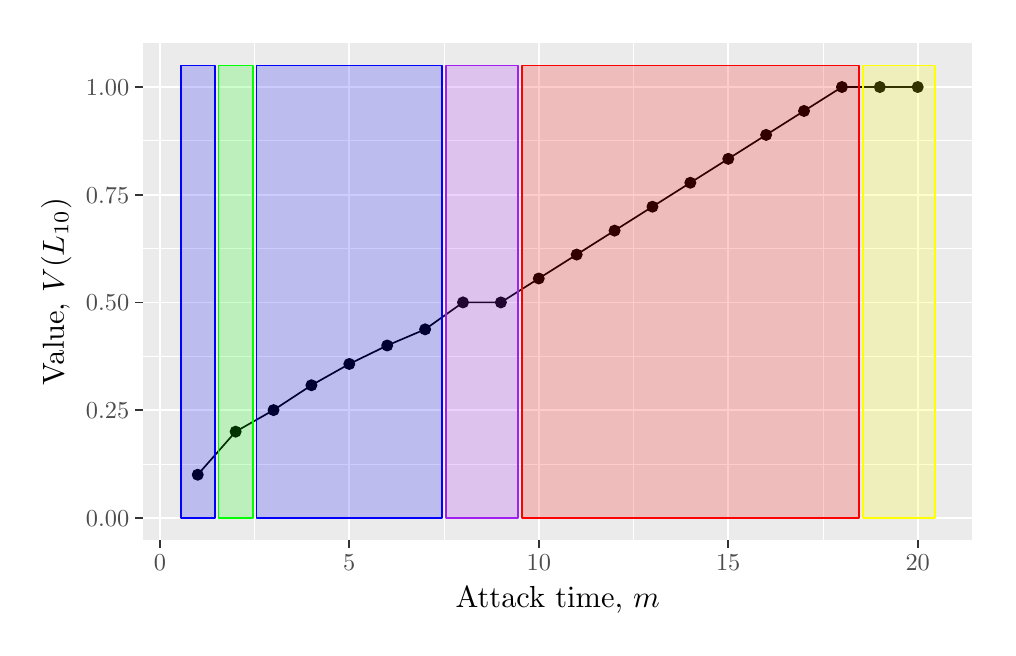
\begin{tikzpicture}[x=1pt,y=1pt]
\definecolor{fillColor}{RGB}{255,255,255}
\path[use as bounding box,fill=fillColor,fill opacity=0.00] (0,0) rectangle (346.90,216.81);
\begin{scope}
\path[clip] (  0.00,  0.00) rectangle (346.90,216.81);
\definecolor{drawColor}{RGB}{255,255,255}
\definecolor{fillColor}{RGB}{255,255,255}

\path[draw=drawColor,line width= 0.6pt,line join=round,line cap=round,fill=fillColor] (  0.00,  0.00) rectangle (346.90,216.81);
\end{scope}
\begin{scope}
\path[clip] ( 41.67, 31.53) rectangle (341.40,211.31);
\definecolor{fillColor}{gray}{0.92}

\path[fill=fillColor] ( 41.67, 31.53) rectangle (341.40,211.31);
\definecolor{drawColor}{RGB}{255,255,255}

\path[draw=drawColor,line width= 0.3pt,line join=round] ( 41.67, 59.16) --
	(341.40, 59.16);

\path[draw=drawColor,line width= 0.3pt,line join=round] ( 41.67, 98.07) --
	(341.40, 98.07);

\path[draw=drawColor,line width= 0.3pt,line join=round] ( 41.67,136.99) --
	(341.40,136.99);

\path[draw=drawColor,line width= 0.3pt,line join=round] ( 41.67,175.90) --
	(341.40,175.90);

\path[draw=drawColor,line width= 0.3pt,line join=round] ( 81.99, 31.53) --
	( 81.99,211.31);

\path[draw=drawColor,line width= 0.3pt,line join=round] (150.45, 31.53) --
	(150.45,211.31);

\path[draw=drawColor,line width= 0.3pt,line join=round] (218.92, 31.53) --
	(218.92,211.31);

\path[draw=drawColor,line width= 0.3pt,line join=round] (287.38, 31.53) --
	(287.38,211.31);

\path[draw=drawColor,line width= 0.6pt,line join=round] ( 41.67, 39.70) --
	(341.40, 39.70);

\path[draw=drawColor,line width= 0.6pt,line join=round] ( 41.67, 78.62) --
	(341.40, 78.62);

\path[draw=drawColor,line width= 0.6pt,line join=round] ( 41.67,117.53) --
	(341.40,117.53);

\path[draw=drawColor,line width= 0.6pt,line join=round] ( 41.67,156.44) --
	(341.40,156.44);

\path[draw=drawColor,line width= 0.6pt,line join=round] ( 41.67,195.36) --
	(341.40,195.36);

\path[draw=drawColor,line width= 0.6pt,line join=round] ( 47.76, 31.53) --
	( 47.76,211.31);

\path[draw=drawColor,line width= 0.6pt,line join=round] (116.22, 31.53) --
	(116.22,211.31);

\path[draw=drawColor,line width= 0.6pt,line join=round] (184.68, 31.53) --
	(184.68,211.31);

\path[draw=drawColor,line width= 0.6pt,line join=round] (253.15, 31.53) --
	(253.15,211.31);

\path[draw=drawColor,line width= 0.6pt,line join=round] (321.61, 31.53) --
	(321.61,211.31);
\definecolor{drawColor}{RGB}{0,0,0}
\definecolor{fillColor}{RGB}{0,0,0}

\path[draw=drawColor,line width= 0.4pt,line join=round,line cap=round,fill=fillColor] (307.92,195.36) circle (  1.96);

\path[draw=drawColor,line width= 0.4pt,line join=round,line cap=round,fill=fillColor] (321.61,195.36) circle (  1.96);

\path[draw=drawColor,line width= 0.4pt,line join=round,line cap=round,fill=fillColor] (184.68,126.18) circle (  1.96);

\path[draw=drawColor,line width= 0.4pt,line join=round,line cap=round,fill=fillColor] (198.38,134.82) circle (  1.96);

\path[draw=drawColor,line width= 0.4pt,line join=round,line cap=round,fill=fillColor] (212.07,143.47) circle (  1.96);

\path[draw=drawColor,line width= 0.4pt,line join=round,line cap=round,fill=fillColor] (225.76,152.12) circle (  1.96);

\path[draw=drawColor,line width= 0.4pt,line join=round,line cap=round,fill=fillColor] (239.45,160.77) circle (  1.96);

\path[draw=drawColor,line width= 0.4pt,line join=round,line cap=round,fill=fillColor] (253.15,169.41) circle (  1.96);

\path[draw=drawColor,line width= 0.4pt,line join=round,line cap=round,fill=fillColor] (266.84,178.06) circle (  1.96);

\path[draw=drawColor,line width= 0.4pt,line join=round,line cap=round,fill=fillColor] (280.53,186.71) circle (  1.96);

\path[draw=drawColor,line width= 0.4pt,line join=round,line cap=round,fill=fillColor] (294.23,195.36) circle (  1.96);

\path[draw=drawColor,line width= 0.4pt,line join=round,line cap=round,fill=fillColor] ( 75.14, 70.83) circle (  1.96);

\path[draw=drawColor,line width= 0.4pt,line join=round,line cap=round,fill=fillColor] (170.99,117.53) circle (  1.96);

\path[draw=drawColor,line width= 0.4pt,line join=round,line cap=round,fill=fillColor] (157.30,117.53) circle (  1.96);

\path[draw=drawColor,line width= 0.4pt,line join=round,line cap=round,fill=fillColor] ( 88.84, 78.62) circle (  1.96);

\path[draw=drawColor,line width= 0.4pt,line join=round,line cap=round,fill=fillColor] (102.53, 87.60) circle (  1.96);

\path[draw=drawColor,line width= 0.4pt,line join=round,line cap=round,fill=fillColor] (116.22, 95.29) circle (  1.96);

\path[draw=drawColor,line width= 0.4pt,line join=round,line cap=round,fill=fillColor] (129.91,101.96) circle (  1.96);

\path[draw=drawColor,line width= 0.4pt,line join=round,line cap=round,fill=fillColor] (143.61,107.80) circle (  1.96);

\path[draw=drawColor,line width= 0.4pt,line join=round,line cap=round,fill=fillColor] ( 61.45, 55.27) circle (  1.96);

\path[draw=drawColor,line width= 0.6pt,line join=round] ( 61.45, 55.27) --
	( 75.14, 70.83) --
	( 88.84, 78.62) --
	(102.53, 87.60) --
	(116.22, 95.29) --
	(129.91,101.96) --
	(143.61,107.80) --
	(157.30,117.53) --
	(170.99,117.53) --
	(184.68,126.18) --
	(198.38,134.82) --
	(212.07,143.47) --
	(225.76,152.12) --
	(239.45,160.77) --
	(253.15,169.41) --
	(266.84,178.06) --
	(280.53,186.71) --
	(294.23,195.36) --
	(307.92,195.36) --
	(321.61,195.36);
\definecolor{drawColor}{RGB}{255,255,0}
\definecolor{fillColor}{RGB}{255,255,0}

\path[draw=drawColor,line width= 0.6pt,line join=round,fill=fillColor,fill opacity=0.20] (301.76, 39.70) rectangle (327.77,203.14);
\definecolor{drawColor}{RGB}{255,0,0}
\definecolor{fillColor}{RGB}{255,0,0}

\path[draw=drawColor,line width= 0.6pt,line join=round,fill=fillColor,fill opacity=0.20] (178.52, 39.70) rectangle (300.39,203.14);
\definecolor{drawColor}{RGB}{160,32,240}
\definecolor{fillColor}{RGB}{160,32,240}

\path[draw=drawColor,line width= 0.6pt,line join=round,fill=fillColor,fill opacity=0.20] (151.14, 39.70) rectangle (177.15,203.14);
\definecolor{drawColor}{RGB}{0,0,255}
\definecolor{fillColor}{RGB}{0,0,255}

\path[draw=drawColor,line width= 0.6pt,line join=round,fill=fillColor,fill opacity=0.20] ( 82.68, 39.70) rectangle (149.77,203.14);
\definecolor{drawColor}{RGB}{0,255,0}
\definecolor{fillColor}{RGB}{0,255,0}

\path[draw=drawColor,line width= 0.6pt,line join=round,fill=fillColor,fill opacity=0.20] ( 68.98, 39.70) rectangle ( 81.31,203.14);
\definecolor{drawColor}{RGB}{0,0,255}
\definecolor{fillColor}{RGB}{0,0,255}

\path[draw=drawColor,line width= 0.6pt,line join=round,fill=fillColor,fill opacity=0.20] ( 55.29, 39.70) rectangle ( 67.61,203.14);
\end{scope}
\begin{scope}
\path[clip] (  0.00,  0.00) rectangle (346.90,216.81);
\definecolor{drawColor}{gray}{0.30}

\node[text=drawColor,anchor=base east,inner sep=0pt, outer sep=0pt, scale=  0.88] at ( 36.72, 36.67) {0.00};

\node[text=drawColor,anchor=base east,inner sep=0pt, outer sep=0pt, scale=  0.88] at ( 36.72, 75.59) {0.25};

\node[text=drawColor,anchor=base east,inner sep=0pt, outer sep=0pt, scale=  0.88] at ( 36.72,114.50) {0.50};

\node[text=drawColor,anchor=base east,inner sep=0pt, outer sep=0pt, scale=  0.88] at ( 36.72,153.41) {0.75};

\node[text=drawColor,anchor=base east,inner sep=0pt, outer sep=0pt, scale=  0.88] at ( 36.72,192.33) {1.00};
\end{scope}
\begin{scope}
\path[clip] (  0.00,  0.00) rectangle (346.90,216.81);
\definecolor{drawColor}{gray}{0.20}

\path[draw=drawColor,line width= 0.6pt,line join=round] ( 38.92, 39.70) --
	( 41.67, 39.70);

\path[draw=drawColor,line width= 0.6pt,line join=round] ( 38.92, 78.62) --
	( 41.67, 78.62);

\path[draw=drawColor,line width= 0.6pt,line join=round] ( 38.92,117.53) --
	( 41.67,117.53);

\path[draw=drawColor,line width= 0.6pt,line join=round] ( 38.92,156.44) --
	( 41.67,156.44);

\path[draw=drawColor,line width= 0.6pt,line join=round] ( 38.92,195.36) --
	( 41.67,195.36);
\end{scope}
\begin{scope}
\path[clip] (  0.00,  0.00) rectangle (346.90,216.81);
\definecolor{drawColor}{gray}{0.20}

\path[draw=drawColor,line width= 0.6pt,line join=round] ( 47.76, 28.78) --
	( 47.76, 31.53);

\path[draw=drawColor,line width= 0.6pt,line join=round] (116.22, 28.78) --
	(116.22, 31.53);

\path[draw=drawColor,line width= 0.6pt,line join=round] (184.68, 28.78) --
	(184.68, 31.53);

\path[draw=drawColor,line width= 0.6pt,line join=round] (253.15, 28.78) --
	(253.15, 31.53);

\path[draw=drawColor,line width= 0.6pt,line join=round] (321.61, 28.78) --
	(321.61, 31.53);
\end{scope}
\begin{scope}
\path[clip] (  0.00,  0.00) rectangle (346.90,216.81);
\definecolor{drawColor}{gray}{0.30}

\node[text=drawColor,anchor=base,inner sep=0pt, outer sep=0pt, scale=  0.88] at ( 47.76, 20.52) {0};

\node[text=drawColor,anchor=base,inner sep=0pt, outer sep=0pt, scale=  0.88] at (116.22, 20.52) {5};

\node[text=drawColor,anchor=base,inner sep=0pt, outer sep=0pt, scale=  0.88] at (184.68, 20.52) {10};

\node[text=drawColor,anchor=base,inner sep=0pt, outer sep=0pt, scale=  0.88] at (253.15, 20.52) {15};

\node[text=drawColor,anchor=base,inner sep=0pt, outer sep=0pt, scale=  0.88] at (321.61, 20.52) {20};
\end{scope}
\begin{scope}
\path[clip] (  0.00,  0.00) rectangle (346.90,216.81);
\definecolor{drawColor}{RGB}{0,0,0}

\node[text=drawColor,anchor=base,inner sep=0pt, outer sep=0pt, scale=  1.10] at (191.53,  7.44) {Attack time, $m$};
\end{scope}
\begin{scope}
\path[clip] (  0.00,  0.00) rectangle (346.90,216.81);
\definecolor{drawColor}{RGB}{0,0,0}

\node[text=drawColor,rotate= 90.00,anchor=base,inner sep=0pt, outer sep=0pt, scale=  1.10] at ( 13.08,121.42) {Value, $V(L_{ 10 })$};
\end{scope}
\end{tikzpicture}
